\documentclass[a4paper,12pt]{article}
\usepackage[a4paper, total={6in, 9in}]{geometry}
\usepackage{amsmath,amsfonts,euscript,times,harvard,color,fancyhdr,float}
\usepackage[backend=biblatex, bibstyle=authoryear, style=numeric,sorting=none]{biblatex}

% \usepackage[backend=biber]{biblatex-chicago}
\bibliography{bibliography}
\usepackage[pdflatex]{graphicx}
\usepackage{hyperref}
\usepackage{graphicx}

\graphicspath{ {./images/} }


\title{Techniques for group-wise feature selection and estimation}
\date{}
\author{
\\
\\
Aditya Chindhade
\\ Carnegie Mellon University
\\ Master's Project Report
\\ 2018
\\
\\
\\Advisor: Prof. Nikolaos V. Sahindis 
}
\begin{document}
	\pagenumbering{gobble}
	\maketitle

	\newpage
	\tableofcontents 
		\newpage
	\listoffigures
	\listoftables

	\newpage
	\pagenumbering{arabic}
	\section{Abstract}
	This work presents the group-wise feature selection and constrained regression capabilities of ALAMO, an algebraic modeling framework developed at the Sahinidis Optimization group, Carnegie Mellon University and comparative benchmarks with popular feature selection techniques. Group-wise feature selection techniques are particularly useful for incorporating prior knowledge about the structure of features in terms of hierarchy and group-wise dependence in the model building process. The uniqueness of the approach is the superior control in terms of specifying groups of features and complex relationships between them, thereby allowing the modeler to define complex relationships among predictors and predictor groups.	The algebraic model resulting from this approach contains fewer terms as compared to Generalized Linear Models (GLMs), thus minimizing generalization error and achieving higher model interpretability. Utilizing an iterative adaptive sampling approach optimized by internal derivative-free optimization solvers, this approach utilizes the subset-selection technique to find the feature subset that best fits the data. The constrained regression methodology in ALAMO is compared with popular modeling techniques such as linear regression, ridge, lasso, elastic-net and group lasso by fitting these models to the low birth weight dataset, a popular dataset for identifying maternal risk-factors affecting the weight of an infant. Basic feature transformations lead to group-wise structure among the features, thus necessitating a group-wise feature selection approach.
	\newpage
	\section{Introduction}
	Some of the major challenges in machine learning approaches include overfitting, high dimensionality and lack of interpretability. The aim of regularization is to reduce overfitting by either feature selection or shrinkage of predictor coefficients. Feature selection techniques also aim to incorporate model interpretability by setting the coefficients of certain predictors to zero, thereby excluding the entire term from the model. This technique, known as sparsity-based regularization, leads to faster computation, dimensionality reduction and improving model interpretability. \\
\\
The first regularization technique dates back to 1970, when Hoerl etal.\cite{hoerl1970ridge} included the $\ell_2$ norm of the coefficients in the ordinary least-squares (OLS) regression problem to shrink the coefficients of the regression solution. This technique is also known as the ridge.
\\\\
The Lasso\cite{tibshirani1996regression} technique was invented in 1996 and became one the highest cited papers in modern statistics and machine learning. Unlike the ridge which aims at shrinking individual coefficients in the regression problem, the lasso acts as a variable selection tool by including the $\ell_1$ norm of the coefficient vector in the OLS objective function. \\\\
The elastic net, formulated in 2005 \cite{zou2005regularization} aims at achieving a balance between the ridge and the lasso by including both, the $\ell_1$ and $\ell_2$ norms of the coefficient vector in the least-squares objective function. Thus, this is a tool that leads to  The elastic net has quickly grown to become a popular tool in modeling financial modeling due to its unique functionality \cite{kim2014forecasting}.\\ \\
Yuan and Lin \cite{yuan2006model} invented the group-lasso technique for selection of feature groups and shrinkage of coefficients within selected feature groups. The model has been referenced in highly cited articles \cite{hastie2009unsupervised,boyd2011distributed} and has secured a unique position in the statistical machine learning community, owing to its fundamental nature and utility. \\\\
The best-subset selection\cite{narendra1977branch,john1994irrelevant,kohavi1997wrappers} technique involves an exhaustive evaluation of all feature subsets to find the model that best fits the data according to a certain error metric. The best-subset selection has been widely regarded as the holy grail of statistics but is feared by computer scientists and modelers due to its intractable nature.\\\\
ALAMO\cite{cozad2014learning,cozad2015combined,wilson2017alamo} is an adaptive-sampling based algebraic modeling framework that utilizes derivative-free optimization techniques for minimizing various error criteria to come up with the simplest model.\\\\
The following sections describe each of these models in detail and experiments for constrained regression using ALAMO.


\newpage
\section{Regularization and feature selection}
This section includes an overview of popular regularization methods and their relationship with feature selection and shrinkage.
\subsection{The Ridge}
\begin{figure}[H]
    \centering
    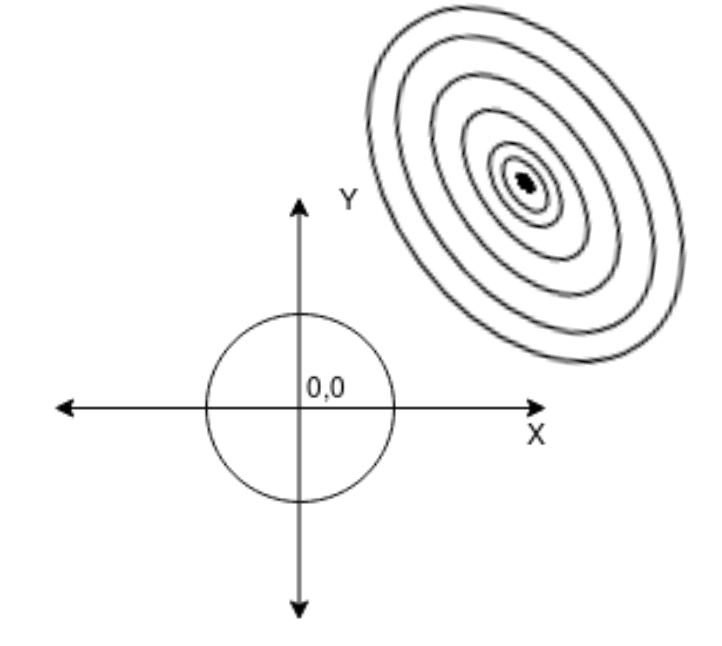
\includegraphics[scale=0.4]{ridge.png}
    \caption{The ridge penalty as a constrained minimization problem}
    \label{fig:ALAMO Flowchart}
\end{figure}
\\
The ridge was formalized in 1970 by Hoerl et al.\cite{hoerl1970ridge} and it seeks to minimize the following objective function:

\begin{eqnarray}
\label{eq:6}
\min_{\beta\in R^p}\left(|| \textbf{y}-\beta_0\one-\sum_{j=1}^J
\textbf{X}_j\beta_j||_2^2 + \lambda ||\vec{\beta}||_2^2 \right)
\end{eqnarray}
In the above equation, \textbf{y} is the target variable vector, $\beta_0$ is the intercept, \textbf{X} is the design matrix, $J$ is the number of predictors, $\vec{\beta}$ is the coefficient vector and $\lambda$ is the regularization parameter. The objective function includes the $\ell_2$ norm of the coefficient vector and is responsible for shrinkage of coefficients. The degree of shrinkage is controlled by the regularization parameter $\lambda$. The ridge is a convex penalty and hence is tractable. The primary use of the ridge penalty is to shrink coefficients to reduce overfitting and thus minimize generalization error\cite{saunders1998ridge}. 


\newpage
\subsection{The Lasso}

\begin{figure}[H]
    \centering
    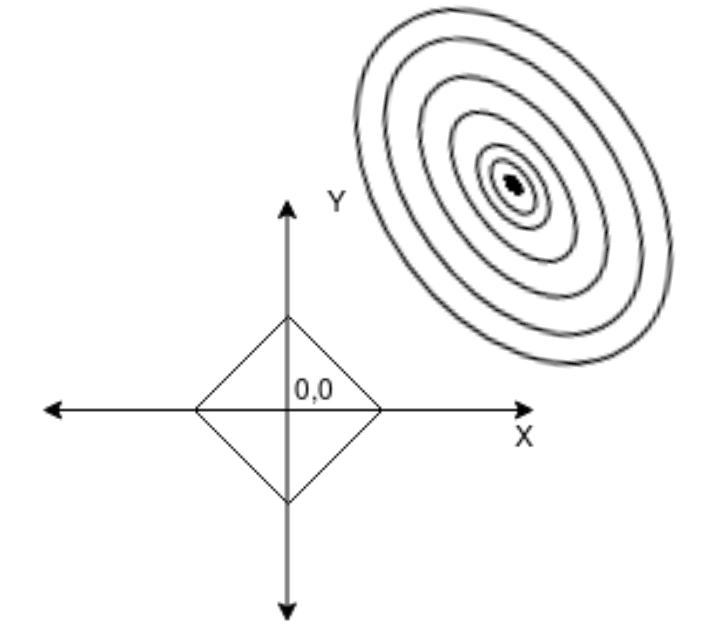
\includegraphics[scale=0.4]{lasso.png}
    \caption{The lasso penalty as a constrained minimization problem}
    \label{fig:ALAMO Flowchart}
\end{figure}

The lasso, formalized in 1996 by Tibshirani et al.\cite{tibshirani1996regression} is a technique to select features by selectively setting predictor coefficients to zero. The formal definition of the lasso penalty is as follows:

\begin{eqnarray}
\label{eq:6}
\min_{\beta\in R^p}\left(|| \textbf{y}-\beta_0\one-\sum_{j=1}^J
\textbf{X}_j\beta_j||_2^2 + \lambda ||\vec{\beta}||_1 \right)
\end{eqnarray}
Similar to the representation for the ridge, \textbf{y} denotes the target variable vector, $\beta_0$ denotes the intercept, \textbf{X} denotes the design matrix, $J$ denotes the number of predictors, $\vec{\beta}$ denotes the coefficient vector and $\lambda$ denotes the regularization parameter. Here, instead of the $\ell_2$ norm, the objective function includes the $\ell_1$ norm of the coefficient vector. This leads to setting individual coefficients to exactly zero along the lasso solution path and hence is used responsible for feature selection. The regularization parameter $\lambda$ governs the degree to which coefficients are penalized; severe penalization leads to a very sparse model, leading to a high bias model, whereas very low penalization may lead to overfitting and a high generalization error. Like the ridge, the lasso is also a convex penalty and hence is tractable. The lasso has applications in feature selection and in reducing overfitting. 



\newpage
\subsection{The Elastic Net}

\begin{figure}[H]
    \centering
    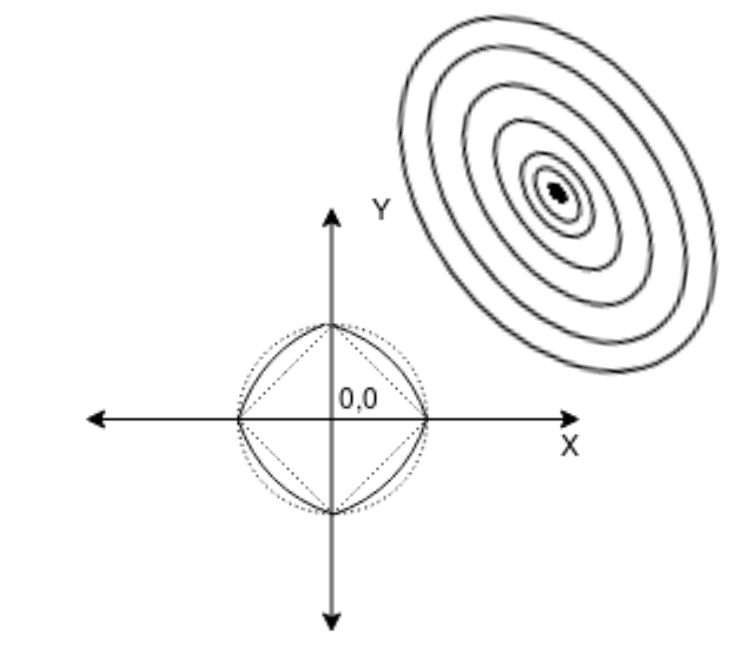
\includegraphics[scale=0.4]{elastic-net.png}
    \caption{The elastic net penalty as a constrained minimization problem}
    \label{fig:ALAMO Flowchart}
\end{figure}
The elastic net  can be considered  as an intermediate between the ridge and the lasso, addressing the shrinkage and variable selection problems simultaneously. The definition of the elastic net problem is as follows:
\begin{eqnarray}
\label{eq:6}
\min_{\beta\in R^p}\left(|| \textbf{y}-\beta_0\one-\sum_{j=1}^J
\textbf{X}_j\beta_j||_2^2 + \lambda_1 ||\vec{\beta}||_1 + \lambda_2 ||\vec{\beta}||_2^2 \right)
\end{eqnarray}
This representation is quite similar to those of the ridge and the lasso with the difference being that here two different penalty terms are included, instead of one. In the above equation, \textbf{y} denotes the target variable vector, $\beta_0$ denotes the intercept, \textbf{X} denotes the design matrix, $J$ denotes the number of predictors, $\vec{\beta}$ denotes the coefficient vector and $\lambda_1$ denotes the regularization parameter for the $\ell_1$ norm and $\lambda_2$ denotes the regularization parameter for the $\ell_2$ norm. Alternatively, the two parameters can also be expressed as one parameter defining the ratio between ridge and lasso and another parameter defining the severity of the overall penalty. While the elastic net accounts for shrinkage and selection, it disregards the group-wise structure and relationships between predictors.
\newpage
\subsection{The Group-Lasso}

\begin{figure}[H]
    \centering
    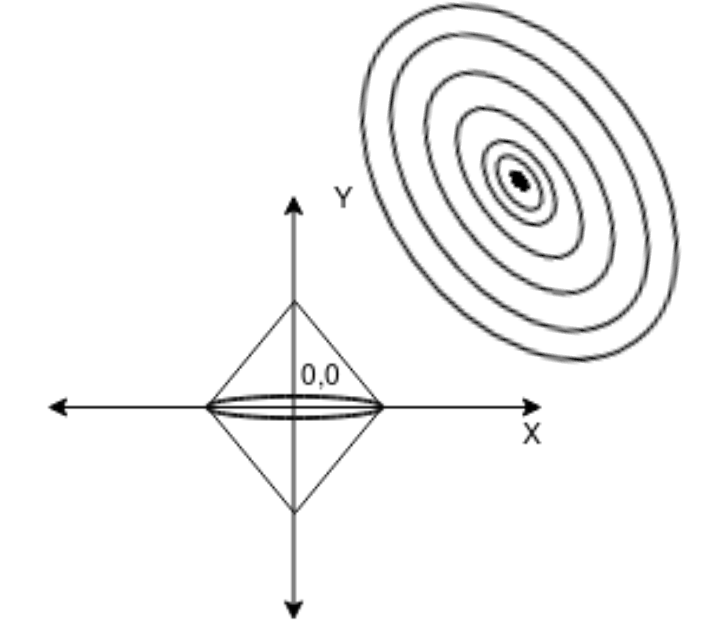
\includegraphics[scale=0.4]{group-lasso.png}
    \caption{The group lasso penalty as a constrained minimization problem}
    \label{fig:ALAMO Flowchart}
\end{figure}


The group lasso was formulated in 2006 by Yuan and Lin \cite{yuan2006model} and has become widely popular as a technique for selecting feature groups. The mathematical formulation of the group lasso is as follows:
\begin{eqnarray}
\min_{\beta\in R^p}\left(|| \textbf{y}-\beta_0\one-\sum_{j=1}^J
\textbf{X}_j\beta_j||_2^2 +\lambda \sum_{\ell=1}^L\sqrt{p_\ell} ||\vec{\beta_\ell}||_2\right)
\label{LM.grlasdef}
\end{eqnarray}

\noindent In this representation, \textbf{y} is the target variable,  \textbf{X} is the feature matrix, $\beta_\00$  is the weight of the bias term and  \vec{$\beta_\ell$}  is the subvector corresponding to the coefficients of variables occurring within the group $\ell$. Here, $J$ is the number of predictors and $L$ is the number of predictor-groups. $\lambda$ is the overall tuning parameter for the group lasso and $\sqrt{p_\ell}$ is the penalty proportional to the size (number of terms) in each group $\ell$. This ensures  normalizing the penalty according to the size of a group. The $\ell_2$ penalty is applied within a group to reduce the magnitude of each of the weights within a group. These norms, being positive are directly added up and effectively work as an $\ell_1$ norm across the groups of weights. This $\ell_1$ is leads to sparsity among feature groups. Thus, the group-lasso can be considered as a two-step penalty. The outer ($\ell_1$) penalty is responsible for selecting feature groups and the inner ($\ell_2$) penalty is responsible for coefficient shrinkage within the selected feature groups.

\newpage
\subsection{Best subset selection}

\begin{figure}[H]
    \centering
    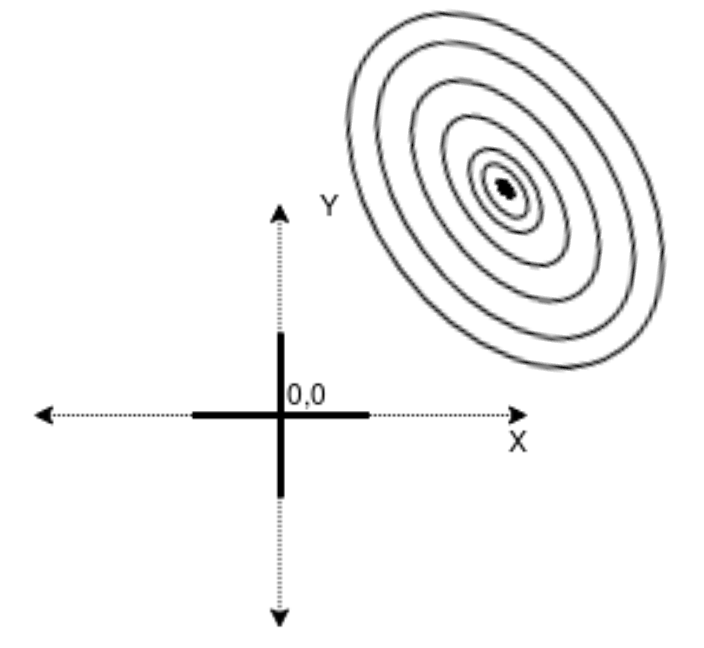
\includegraphics[scale=0.4]{best-subset.png}
    \caption{The best-subset selection technique}
    \label{fig:ALAMO Flowchart}
\end{figure}

The best-subset technique \cite{narendra1977branch,john1994irrelevant,kohavi1997wrappers} was first formalized in 1977 and as a technique for feature selection and is essentially an exhaustive search across all feature subsets to find the feature subset that minimizes the loss function with respect to the features vector consisting of the feature subset selected. While this isn't exactly the same as calculating a vector norm, it is known as the $\ell_0$ norm owing to the effective feature set obtained. Each feature can either be included in the model or excluded from it. This leads to the following relation:

\begin{eqnarray}
\textrm{Number of subsets} = 2^{\textrm{number of features}}
\end{eqnarray}
Being exponential in the number of features, the best subset selection technique is often considered intractable. However, due to the exhaustive search across feature subsets to find the best subset, this technique is widely considered as the holy grail of statistics and has been of interest lately due to advances in computing and enhancements in memory.


% \newpage
% \subsection{Summary}

% \begin{center}
% \begin{table}[]
% \begin{tabular}{|l|l|l|l|l|}
% \hline
% Technique             & Tractable & Convex & Differentiable     & Norm   \\ \hline
% Ridge                 & Yes       & Yes    & Yes                & L_2     \\ \hline
% Lasso                 & Yes       & Yes    & No                 & L_1     \\ \hline
% Elastic net           & Yes       & Yes    & Depends on penalty & L_1+L_2  \\ \hline
% Group Lasso           & Yes       & Yes    & No                 & L_1(L_2) \\ \hline
% Best subset selection & No        & No     & No                 & L_0     \\ \hline
% \end{tabular}
% \end{table}
% \end{center}

\newpage
\section{ALAMO (Automated Learning of Algebraic Models for Optimization)}
ALAMO \cite{cozad2014learning,cozad2015combined,wilson2017alamo} is a black-box modeling toolbox developed at the Sahinidis Optimization Group, Carnegie Mellon University. ALAMO implements an integer-programming based best-subset selection strategy for variable selection which utilizes the hallowed $\ell_0$ norm for variable selection and solves non-convex the optimization problem using derivative-free optimization solvers. 
\subsection{The ALAMO model-building process}
The ALAMO model-building process consists of two key steps:
\subsubsection{Surrogate Model Generation}
The solution approach begins by sampling an initial set of points from the input data set, which is then used for building an initial model, starting with the lowest complexity. Various combinations of simple basis functions are considered for generating algebraic models, which are then solved using an optimization framework. 
%write more about alamo

\subsubsection{Adaptive Sampling}
Adaptive sampling is an active learning \cite{angluin1988queries,settles.tr09} approach which involves querying the data for selecting the next set of points such that maximum model accuracy can be obtained with minimum additional information. This is done by an error-maximization strategy, which means that the points which have the largest deviation from the model are included in the next sample for model building. 
\subsection{Constrained regression in ALAMO}
ALAMO allows manual specification of constraints on features and includes specification of feature groups. These feature groups could be defined by either polynomial transformations of the same feature forming a group or based on prior knowledge about heirarchical structure within the features. The constraint types are as follows:
\begin{table}[H]
\centering
\begin{tabular}{|c|l|}
\hline
\textbf{Keyword} & \multicolumn{1}{c|}{\textbf{Meaning}}                           \\ \hline
REQ              & If group i is selected, group j is also selected.               \\ \hline
XCL              & If group i is selected, group j is NOT selected and vice-versa. \\ \hline
NMT              & Not more than k variables within group i must be selected.      \\ \hline
ATL              & At least k variables within group i must be selected.           \\ \hline
\end{tabular}
\caption{Constraint types in ALAMO}
 
\end{table}

\newpage

\begin{figure}[H]
 \centering
 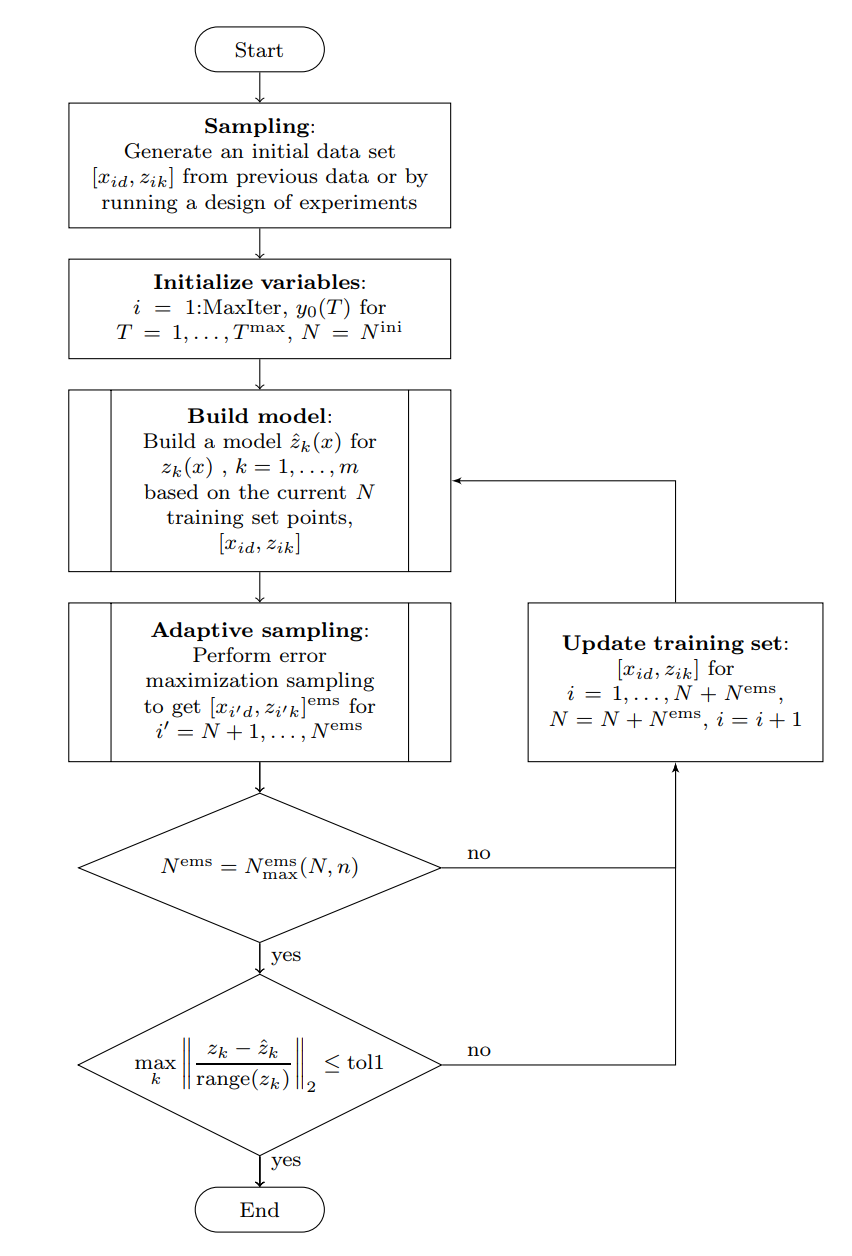
\includegraphics[scale=0.4]{flowchart-alamo.png}
 \caption{The ALAMO approach}
  \label{fig:ALAMO Flowchart}
\end{figure}

\newpage
\section{Experiments}
	\subsection{Dataset description}
		The dataset, popularly known as the low-birth-weight dataset consists of risk factors affecting the weight of a new born child. This dataset was first published in the book - Applied Logistic Regression by Hosmer and Lemeshow \cite{hosmer2013applied} and consists of the  data were collected at Baystate Medical Center, Springfield, Mass during 1986. The data in the raw format can be found in popular repositories like MLData (http://www.mldata.org/repository/data/viewslug/uci-20070111-lowbwt/). The original dataset consists of a real valued target variable-weight of child, with 8 features and 189 data points. The features are as follows:
    


\begin{table}[H]
\centering
\begin{tabular}{|l|c|c|}
\hline
\multicolumn{1}{|c|}{\textbf{Feature}}                 & \textbf{Abbreviation} & \textbf{Data type} \\ \hline
Mother’s age                                           & age                   & continuous         \\ \hline
Mother’s weight                                        & lwt                   & continuous         \\ \hline
Smoking status during pregnancy                        & smoke                 & boolean            \\ \hline
Mother's Race                                          & black/white           & categorical        \\ \hline
Number of premature labors                             & ptl                   & integer            \\ \hline
History of hypertension                                & ht                    & boolean            \\ \hline
History of uterine irritability                        & ui                    & boolean            \\ \hline
Number of clinician visits                             & ftv                   & integer            \\ \hline
\end{tabular}
\caption{Description of features}
\end{table}

\subsection{Feature transformations}
        Additional features corresponding to polynomial transformations of the features have been created. The features age1, age2, age3 correspond to first, second and third order polynomial transformation of the mother's age. Similarly, lwt2, lwt3 are features corresponding to square and cube of the mother's weight. The categorical features have been transformed using one-hot encoding. This transformed dataset is also available in the public domain for analysis.
        
    \subsubsection{Feature grouping}
        Feature groups are identified based on either polynomial transformations of the same primary variable or prior knowledge about association between features. For example, features age1, age2, age3 and features lwt1, lwt2, lwt3 form 2 groups based on polynomial transformations. Additionally, features corresponding to either one or more than one premature labors form a group and those corresponding to either one, two or more than two physician visits in the first trimester form another group. Lastly, one-hot encodings of a categorical variable form a group. The feature groups can be seen in the representation below:
\begin{figure}[H]
\centering
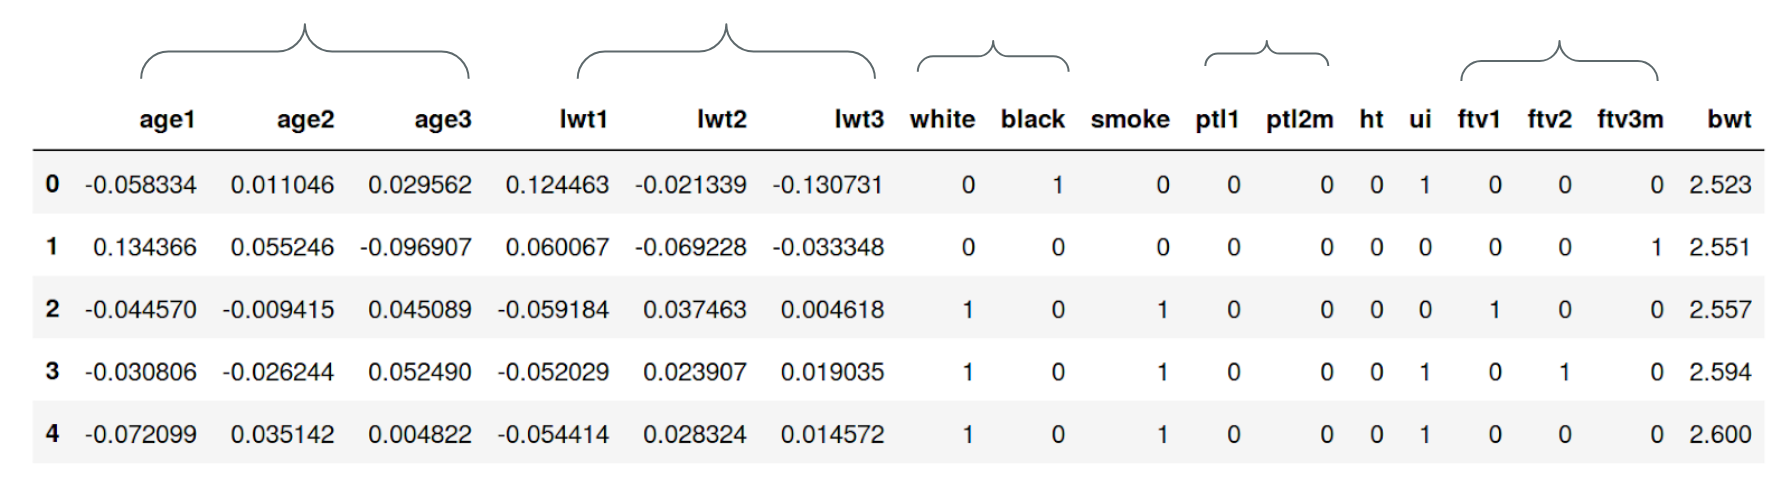
\includegraphics[scale=0.25]{feature-grouping.png}
\caption{Identification of feature groups}
\label{fig:ALAMO Flowchart}
\end{figure}

        
        
\subsection{Correlation plot}
Pearson correlation between each predictor and the target variable is plotted. The correlations can be seen as follows:

    \begin{figure}[H]
     \centering
     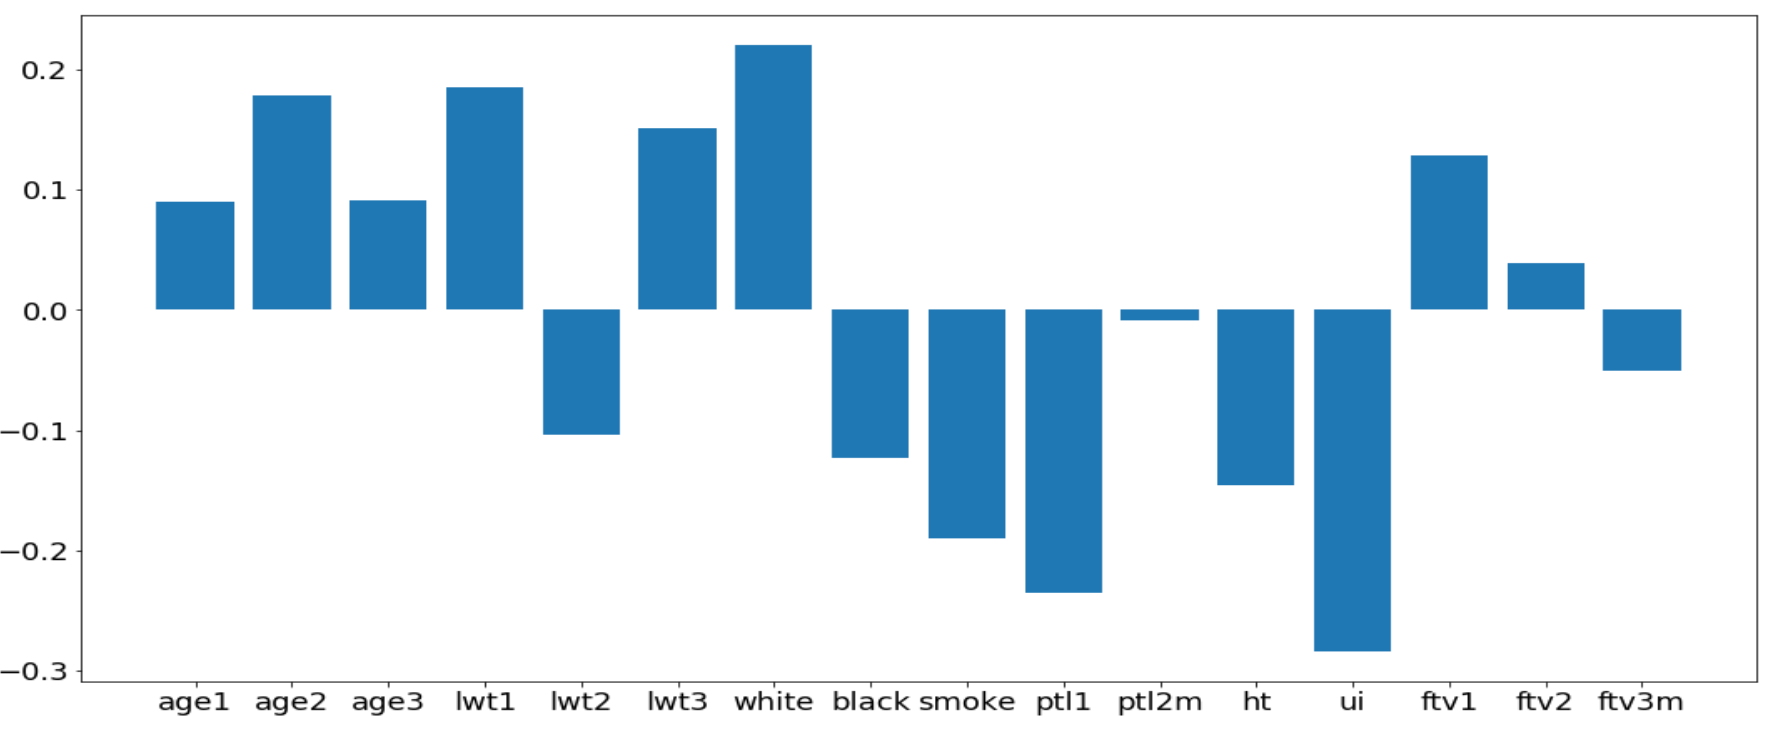
\includegraphics[scale=0.25]{corr.png}
     \caption{Correlation plot: Pearson correlation of each feature with target variable}
      \label{fig:ALAMO Flowchart}
    \end{figure}
    \noindent It can be observed that the variable ptl2m, which corresponds to two or more premature labors is the variable least correlated with the response variable. Similarly, number of clinician visits have relatively low correlations with the response variable, weight. This is intuitive as we do not generally expect the number of times a mother visited the clinic to affect the weight of her new born child.

\newpage
\subsection{Modeling}
    Multiple models such as linear regression, ridge, lasso, elastic net, group-lasso and ALAMO were used for fitting the data and mean-squared error for each model was reported. Additionally, average runtime across 5 runs was measured for all models and reported. All experiments were run on a machine with Intel i7 CPU with 8 cores at 2.9 GHz and 16 GB RAM running 64-bit Ubuntu 18.04.
    \subsubsection{Generalized linear models}
    Generalized linear models such as multiple linear regression, ridge, lasso, elastic net and group-lasso were implemented. The data was shuffled, mean-normalized and a 4-fold cross validation mean-squared error was reported. For regularization models involving a parameter, a parametric sweep was conducted for various values of the tuning parameter and mean-squared errors were plotted. The minimum value of the mean-squared error from each model has been included in the model summary in a later section of this work. Linear regression, ridge, lasso and elastic net models were implemented using the Scikit-learn\cite{scikit-learn} framework in Python and the group lasso was implemented using the grpreg\cite{breheny2015group} package in R.
    \subsubsection{ALAMO}    
    ALAMO version 2018.6.20 was licensed and downloaded from The Optimization Firm website: \href{https://minlp.com/alamo}{www.minlp.com}.
    \\Data and constraints were described in a .alm file. 16 groups were defined corresponding to each of the predictor variables and relationships between the predictors were defined to utilize the constrained regression capability in ALAMO. The group specification for ALAMO is different from that of the group lasso in that each variable is defined as a group entity and relationships between these groups are established. The groups are defined as follows:
\begin{table}[H]
\centering
\begin{tabular}{|c|c|c|}
\hline
\textbf{Group-ID} & \textbf{Member-type} & \textbf{Member-indices} \\ \hline
1                 & lin                  & 1                       \\ \hline
2                 & lin                  & 2                       \\ \hline
3                 & lin                  & 3                       \\ \hline
4                 & lin                  & 4                       \\ \hline
5                 & lin                  & 5                       \\ \hline
6                 & lin                  & 6                       \\ \hline
7                 & lin                  & 7                       \\ \hline
8                 & lin                  & 8                       \\ \hline
9                 & lin                  & 9                       \\ \hline
10                & lin                  & 10                      \\ \hline
11                & lin                  & 11                      \\ \hline
12                & lin                  & 12                      \\ \hline
13                & lin                  & 13                      \\ \hline
14                & lin                  & 14                      \\ \hline
15                & lin                  & 15                      \\ \hline
16                & lin                  & 16                      \\ \hline
\end{tabular}
\caption{Definition of feature groups in ALAMO}
\end{table}
In the above representation the first column specifies the group ID. As each variable is defined as its own group, the group-ID is the same as variable-ID. The keyword lin specifies that only linear basis functions of the group are considered. Lastly, the column member-indices specifies the contents of each group in terms of the group-ID of each member. In this case, as each group contains only 1 variable and the member index is same as group-ID.\\ \\
Group constraints can be specified between the predictors using pre-established relationships between predictors. The constraint definitions are as follows:

\begin{table}[H]
\centering
\begin{tabular}{|c|c|c|c|}
\hline
\textbf{Group-ID} & \textbf{Output-ID} & \textbf{Constraint type} & \textbf{Integer parameter} \\ \hline
1                 & 1                  & atl                      & 1                          \\
1                 & 1                  & req                      & 2                          \\
1                 & 1                  & req                      & 3                          \\
2                 & 1                  & req                      & 1                          \\
2                 & 1                  & req                      & 3                          \\
3                 & 1                  & req                      & 1                          \\
3                 & 1                  & req                      & 2                          \\ \hline
4                 & 1                  & atl                      & 1                          \\
4                 & 1                  & req                      & 5                          \\
4                 & 1                  & req                      & 6                          \\
5                 & 1                  & req                      & 4                          \\
5                 & 1                  & req                      & 6                          \\
6                 & 1                  & req                      & 4                          \\
6                 & 1                  & req                      & 5                          \\ \hline
7                 & 1                  & atl                      & 1                          \\
7                 & 1                  & xcl                      & 8                          \\
8                 & 1                  & xcl                      & 7                          \\ \hline
10                & 1                  & req                      & 11                         \\
11                & 1                  & req                      & 10                         \\ \hline
14                & 1                  & req                      & 15                         \\
15                & 1                  & req                      & 16                         \\
16                & 1                  & req                      & 14                         \\ \hline
\end{tabular}
\caption{Defintion of group-constraints in ALAMO}
\end{table}
\noindent In this representation, group-ID represents the group-ID defined in the group definitions section, output-ID specifies the number of outputs for which the constraint would be imposed. This specification is particularly useful in multivariate linear regression. The constraint-type section defines the type of group-constraint to be utilized. A summary of group constraints can be seen in section 4.3 of this work. Lastly, the integer-parameter column contains the index of the constraint to which the group belongs. As each group could belong to multiple constraints, this column can contain multiple group-ids. In our case, as each inter-group relation is symmetric and transitive, these constraints can also be defined in a cyclic manner: (1 \rightarrow 2, 2 \rightarrow 3, 3 \rightarrow 1).
    
	\newpage
	\section{Results and Discussion}
		\subsection{Linear Regression}
		Linear regression can be considered as the simplest of all the models considered in this work. In this model, a multiple linear regression model is fitted using the data. The coefficients obtained are as follows:
		    \begin{table}[H]
		    \centering
            \begin{tabular}{|l|c|}
            \hline
            \textbf{Feature} & \textbf{Weight} \\ \hline
            age1             & -0.4211         \\ \hline
            age2             & 1.7217          \\ \hline
            age3             & 0.7250          \\ \hline
            lwt1             & 2.3606          \\ \hline
            lwt2             & 0.2525          \\ \hline
            lwt3             & 1.4769          \\ \hline
            white            & 0.1749          \\ \hline
            black            & -0.2669         \\ \hline
            smoke            & -0.2165         \\ \hline
            ptl1             & -0.4291         \\ \hline
            ptl2m            & 0.2897          \\ \hline
            ht               & -0.6244         \\ \hline
            ui               & -0.5241         \\ \hline
            ftv1             & 0.2067          \\ \hline
            ftv2             & -0.0392         \\ \hline
            ftv3m            & -0.1249         \\ \hline
            intercept        & 3.1077          \\ \hline
            mse              & 0.4825          \\ \hline
            \end{tabular}
            \caption{Coefficients obtained from linear regression}
            \end{table}
		\noindent The simplest form of multiple linear regression contains non-zero values for all predictor coefficients, indicating that all terms are included in the model. The 4-fold cross-validation mean-squared error is obtained by as 0.4825. The average overall runtime for linear regression is 5 ms.
		\\\\
		As this model doesn't include any regularization, it tends to overfit on the training data and hence gives a relatively high generalization error. This model can be improved upon by using regularization methods and incorporating group-wise structure among features to build a better model.

		\newpage
		\subsection{Ridge}
		The ridge is a convex penalty responsible for shrinkage of coefficients. The magnitude of the coefficients is determined by $\lambda$, the penalizing coefficient. In the experiment, a parametric sweep across different penalizing coefficient values starting at 0.001 and increasing in steps of multiples of 10 to a value of $\lambda$ = 1000. Average value of coefficients obtained for all predictors from a four-fold cross-validation are plotted against the base-10 log of the penalizing coefficient value. This gives the following graph:
		\begin{figure}[H]
		     \centering
            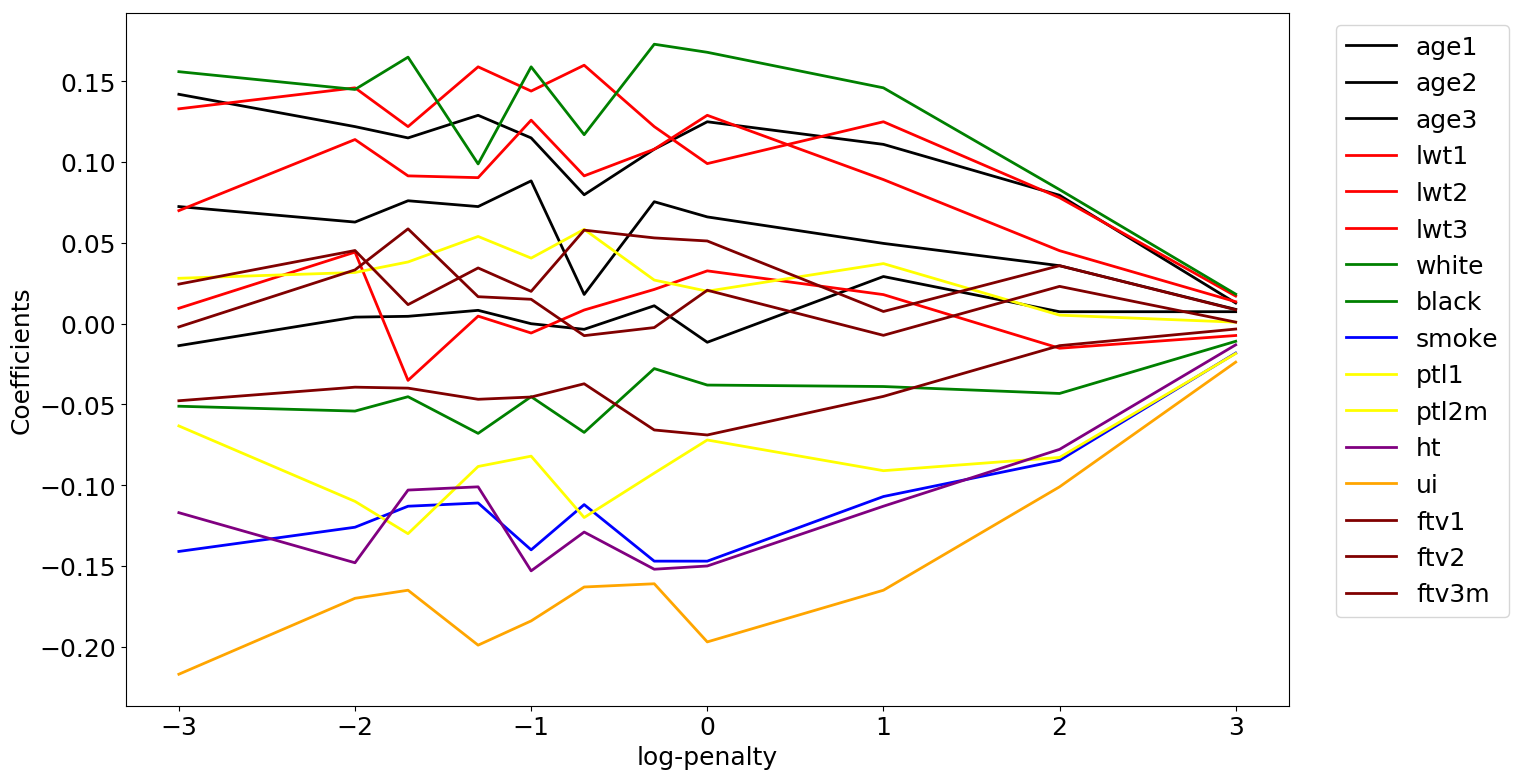
\includegraphics[scale=0.4]{ridge-path.png}
            \caption{Ridge coefficients vs base-10 log of tuning parameter}
        \end{figure}
        
        \noindent In the above graph, the predictors are color-coded according to the groups they belong to. Although it does not affect the ridge penalty this representation is useful in comparing the ridge with group-wise feature selection discussed in a later section. It can be seen that the ridge doesn't set any coefficient to exactly zero, however, as the penalizing coefficient value increases, it can be seen that the magnitude of the coefficients decreases. The value of each coefficient as it varies with the tuning parameter is described in the following table:
        \begin{table}[H]
        \resizebox{\columnwidth}{!}{%
\begin{tabular}{|l|c|c|c|c|c|c|c|c|c|c|c|}
\hline
\textbf{penalty}     & \textbf{0.001} & \textbf{0.01} & \textbf{0.02} & \textbf{0.05} & \textbf{0.10} & \textbf{0.20} & \textbf{0.50} & \textbf{1.00} & \textbf{10.00} & \textbf{100.00} & \textbf{1,000.00} \\ \hline
\textbf{log-penalty} & -3.0000        & -2.0000       & -1.6990       & -1.3010       & -1.0000       & -0.6990       & -0.3010       & 0.0000        & 1.0000         & 2.0000          & 3.0000            \\ \hline
\textbf{age1}        & -0.0136        & 0.0041        & 0.0046        & 0.0083        & 0.0000        & -0.0035       & 0.0111        & -0.0115       & 0.0292         & 0.0074          & 0.0074            \\ \hline
\textbf{age2}        & 0.1416         & 0.1218        & 0.1147        & 0.1286        & 0.1149        & 0.0798        & 0.1083        & 0.1246        & 0.1111         & 0.0795          & 0.0128            \\ \hline
\textbf{age3}        & 0.0725         & 0.0629        & 0.0761        & 0.0725        & 0.0884        & 0.0181        & 0.0755        & 0.0661        & 0.0497         & 0.0359          & 0.0088            \\ \hline
\textbf{lwt1}        & 0.1327         & 0.1459        & 0.1222        & 0.1587        & 0.1438        & 0.1604        & 0.1223        & 0.0991        & 0.1246         & 0.0780          & 0.0171            \\ \hline
\textbf{lwt2}        & 0.0095         & 0.0443        & -0.0351       & 0.0047        & -0.0058       & 0.0085        & 0.0212        & 0.0327        & 0.0180         & -0.0152         & -0.0073           \\ \hline
\textbf{lwt3}        & 0.0700         & 0.1139        & 0.0915        & 0.0904        & 0.1262        & 0.0915        & 0.1083        & 0.1287        & 0.0892         & 0.0452          & 0.0136            \\ \hline
\textbf{white}       & 0.1555         & 0.1448        & 0.1653        & 0.0989        & 0.1585        & 0.1165        & 0.1730        & 0.1680        & 0.1456         & 0.0830          & 0.0183            \\ \hline
\textbf{black}       & -0.0511        & -0.0541       & -0.0452       & -0.0679       & -0.0452       & -0.0673       & -0.0278       & -0.0380       & -0.0389        & -0.0432         & -0.0109           \\ \hline
\textbf{smoke}       & -0.1406        & -0.1262       & -0.1128       & -0.1111       & -0.1400       & -0.1119       & -0.1469       & -0.1472       & -0.1072        & -0.0846         & -0.0182           \\ \hline
\textbf{ptl1}        & -0.0633        & -0.1102       & -0.1301       & -0.0884       & -0.0820       & -0.1196       & -0.0925       & -0.0720       & -0.0910        & -0.0828         & -0.0185           \\ \hline
\textbf{ptl2m}       & 0.0281         & 0.0317        & 0.0382        & 0.0540        & 0.0406        & 0.0584        & 0.0270        & 0.0201        & 0.0372         & 0.0053          & 0.0009            \\ \hline
\textbf{ht}          & -0.1169        & -0.1480       & -0.1028       & -0.1014       & -0.1533       & -0.1288       & -0.1522       & -0.1500       & -0.1133        & -0.0778         & -0.0131           \\ \hline
\textbf{ui}          & -0.2172        & -0.1705       & -0.1654       & -0.1995       & -0.1844       & -0.1633       & -0.1606       & -0.1965       & -0.1647        & -0.1008         & -0.0238           \\ \hline
\textbf{ftv1}        & 0.0245         & 0.0453        & 0.0118        & 0.0345        & 0.0200        & 0.0579        & 0.0531        & 0.0512        & 0.0075         & 0.0359          & 0.0086            \\ \hline
\textbf{ftv2}        & -0.0020        & 0.0333        & 0.0587        & 0.0167        & 0.0151        & -0.0074       & -0.0024       & 0.0207        & -0.0072        & 0.0231          & 0.0010            \\ \hline
\textbf{ftv3m}       & -0.0477        & -0.0393       & -0.0399       & -0.0468       & -0.0454       & -0.0372       & -0.0658       & -0.0689       & -0.0450        & -0.0136         & -0.0033           \\ \hline
\textbf{intercept}   & 2.9643         & 2.9504        & 2.9594        & 2.9589        & 2.9569        & 2.9493        & 2.9661        & 2.9551        & 2.9340         & 2.9552          & 2.9537            \\ \hline
\textbf{mse}         & 0.4543         & 0.4687        & 0.5274        & 0.4634        & 0.4825        & 0.4666        & 0.4725        & 0.5086        & 0.4676         & 0.4235          & 0.4858            \\ \hline
\end{tabular}
}
\caption{Ridge coefficients as a function of tuning parameter}
\end{table}

\\
\noindent We can also plot the mean squared error as a function of the penalizing coefficient $\lambda$. This helps us obtain the following graph:
\begin{figure}[H]
            \centering
            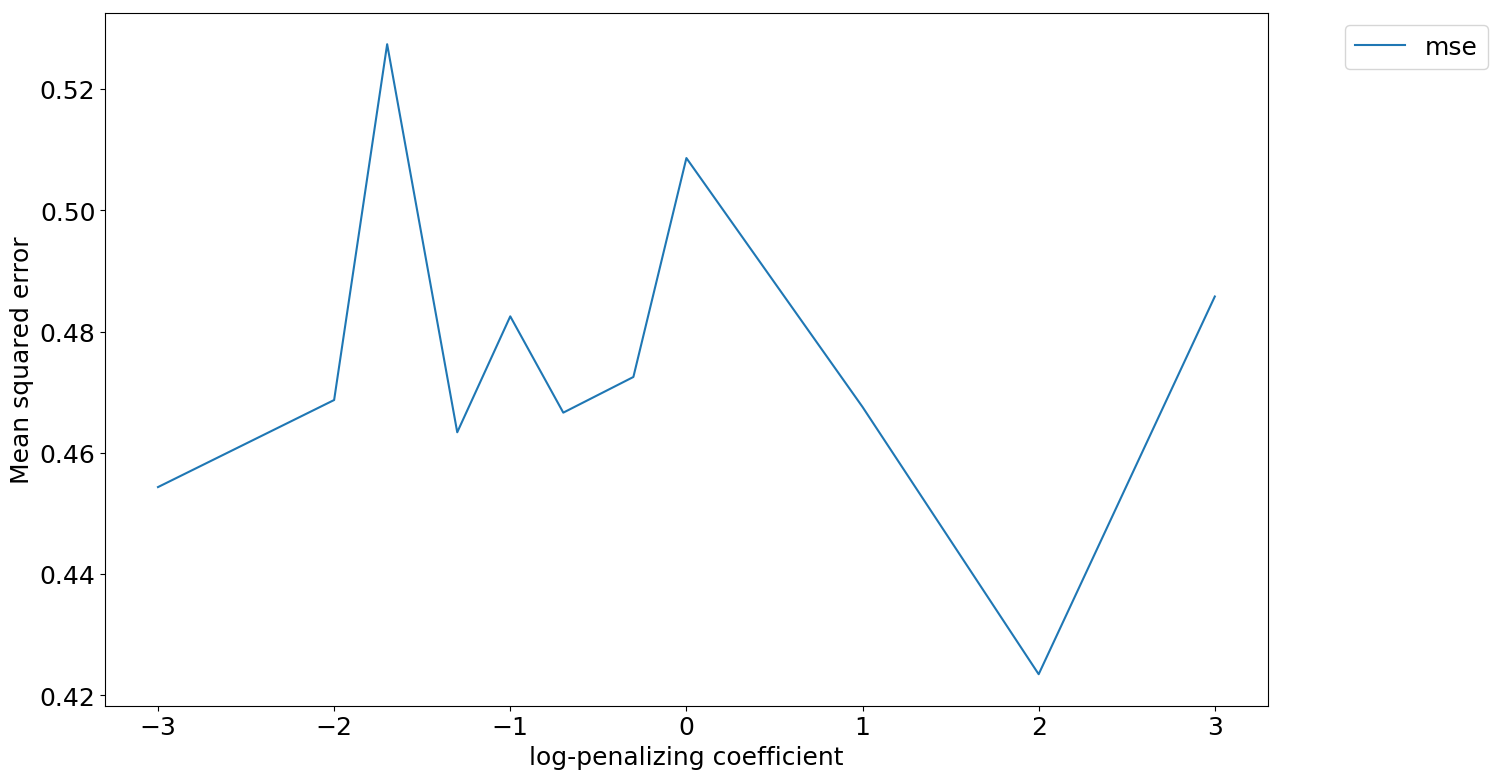
\includegraphics[scale=0.3]{mse-lambda-ridge.png}
            \caption{Ridge mean-squared error vs base-10 log of tuning parameter}
\end{figure}
\noindent We can infer that the lowest value of mean-squared error is obtained when $\lambda$ = 100 and the mean squared error value is 0.4235. This mean squared error is lower than that of linear regression as coefficient shrinkage helps in minimizing generalization error. The average runtime for the ridge is 43.1 ms.

		\newpage
		\subsection{Lasso}
		The lasso is responsible for feature selection by setting the coefficients of predictors in the model to exactly zero, thereby introducing sparsity in the model. This is evident from the results and can be seen by plotting the value of all coefficients as a function of the log base-10 penalizing coefficient.
        \begin{figure}[H]
            \centering
            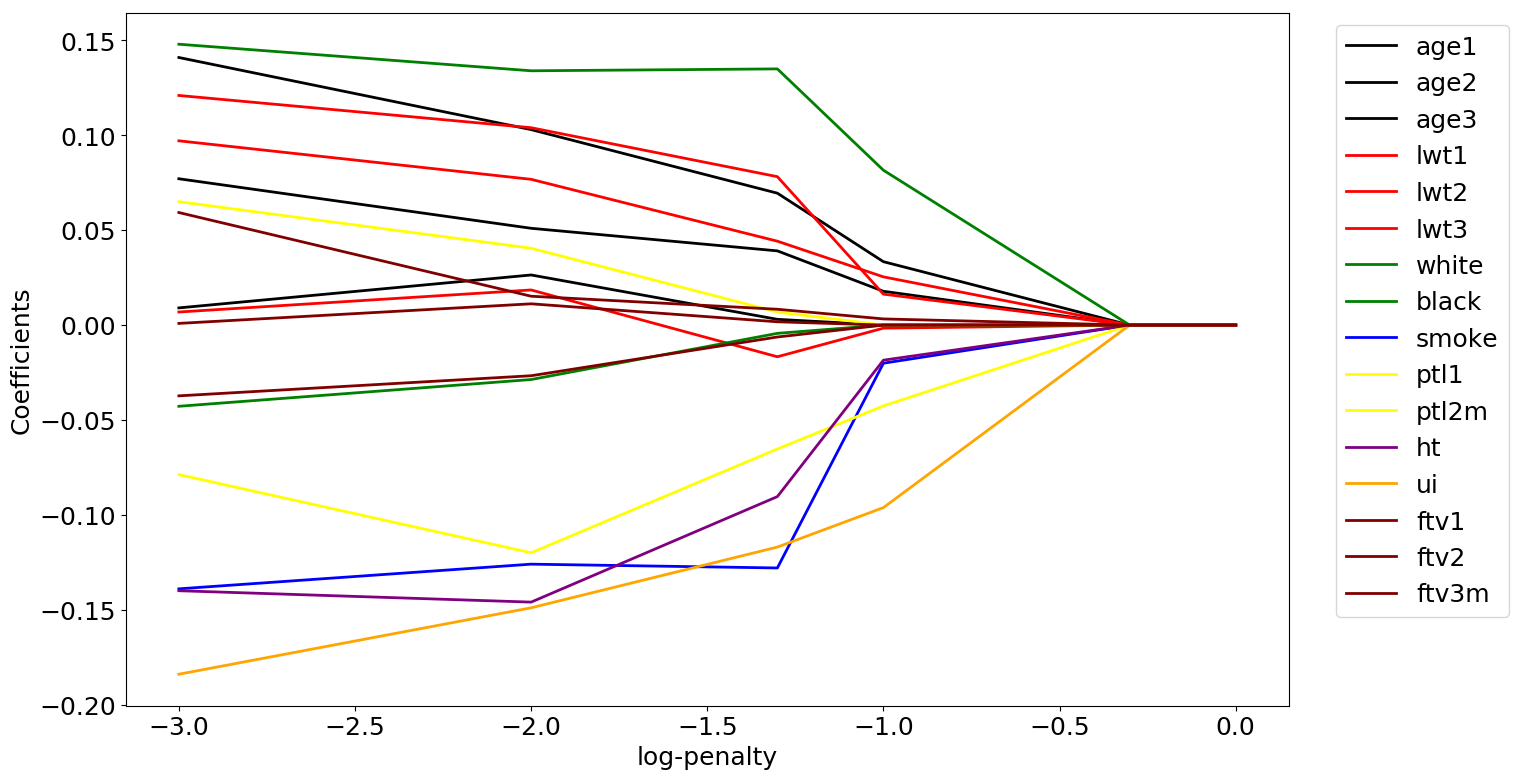
\includegraphics[scale=0.4]{lasso-path.png}
            \caption{Lasso coefficientsvs base-10 log of tuning parameter}
            \label{fig:neurons}
        \end{figure}
        \noindent In the above graph, individual predictors are color-coded according to the group they belong to. From the figure, we can analyze how different coefficients are set to zero as the penalizing coefficient $\lambda$ is increased from 0.0001 to 1 in multiples of 10. The sparsity introduced in the model can further be explained by the following table indicating the coefficients, intercept and mean-squared error as a function of the tuning parameter $\lambda$.
        
        
        
\begin{table}[H]
\centering
\begin{tabular}{|l|c|c|c|c|c|c|c|}
\hline
\textbf{penalty}     & \textbf{0.0001} & \textbf{0.0010} & \textbf{0.0100} & \textbf{0.0500} & \textbf{0.1000} & \textbf{0.5000} & \textbf{1.0000} \\ \hline
\textbf{log-penalty} & -4.0000         & -3.0000         & -2.0000         & -1.3010         & -1.0000         & -0.3010         & 0.0000          \\ \hline
\textbf{age1}        & 0.0430          & 0.0066          & -0.0126         & 0.0000          & 0.0000          & 0.0000          & 0.0000          \\ \hline
\textbf{age2}        & 0.1535          & 0.1303          & 0.0945          & 0.0376          & 0.0317          & 0.0000          & 0.0000          \\ \hline
\textbf{age3}        & 0.1044          & 0.0599          & 0.0541          & 0.0188          & 0.0014          & 0.0000          & 0.0000          \\ \hline
\textbf{lwt1}        & 0.1447          & 0.1352          & 0.1267          & 0.0606          & 0.0364          & 0.0000          & 0.0000          \\ \hline
\textbf{lwt2}        & -0.0254         & -0.0160         & 0.0014          & 0.0000          & -0.0044         & 0.0000          & 0.0000          \\ \hline
\textbf{lwt3}        & 0.1280          & 0.1223          & 0.0901          & 0.0416          & 0.0062          & 0.0000          & 0.0000          \\ \hline
\textbf{white}       & 0.1337          & 0.1363          & 0.1433          & 0.0826          & 0.0582          & 0.0000          & 0.0000          \\ \hline
\textbf{black}       & -0.0769         & -0.0451         & -0.0509         & -0.0132         & 0.0000          & 0.0000          & 0.0000          \\ \hline
\textbf{smoke}       & -0.1508         & -0.1150         & -0.1386         & -0.0867         & -0.0468         & 0.0000          & 0.0000          \\ \hline
\textbf{ptl1}        & -0.0744         & -0.0958         & -0.1088         & -0.0626         & -0.0279         & 0.0000          & 0.0000          \\ \hline
\textbf{ptl2m}       & 0.0625          & 0.0112          & 0.0150          & 0.0000          & 0.0000          & 0.0000          & 0.0000          \\ \hline
\textbf{ht}          & -0.1206         & -0.1322         & -0.1371         & -0.1021         & -0.0177         & 0.0000          & 0.0000          \\ \hline
\textbf{ui}          & -0.1573         & -0.1916         & -0.1545         & -0.1423         & -0.0911         & 0.0000          & 0.0000          \\ \hline
\textbf{ftv1}        & 0.0359          & 0.0310          & 0.0390          & 0.0124          & 0.0027          & 0.0000          & 0.0000          \\ \hline
\textbf{ftv2}        & 0.0442          & 0.0082          & 0.0220          & 0.0000          & 0.0000          & 0.0000          & 0.0000          \\ \hline
\textbf{ftv3m}       & -0.0557         & -0.0337         & -0.0115         & -0.0082         & 0.0000          & 0.0000          & 0.0000          \\ \hline
\textbf{intercept}   & 2.9483          & 2.9403          & 2.9324          & 2.9327          & 2.9535          & 2.9650          & 2.9613          \\ \hline
\textbf{mse}         & 0.4942          & 0.4181          & 0.5108          & 0.5109          & 0.4894          & 0.5483          & 0.4417          \\ \hline
\end{tabular}
\caption{Lasso coefficients as a function of tuning parameter}
\end{table}

\noindent  We can also plot the mean-square error as a function of the base-10 log of the tuning parameter $\lamda$. The graph obtained is as follows:
\begin{figure}[H]
    \centering
    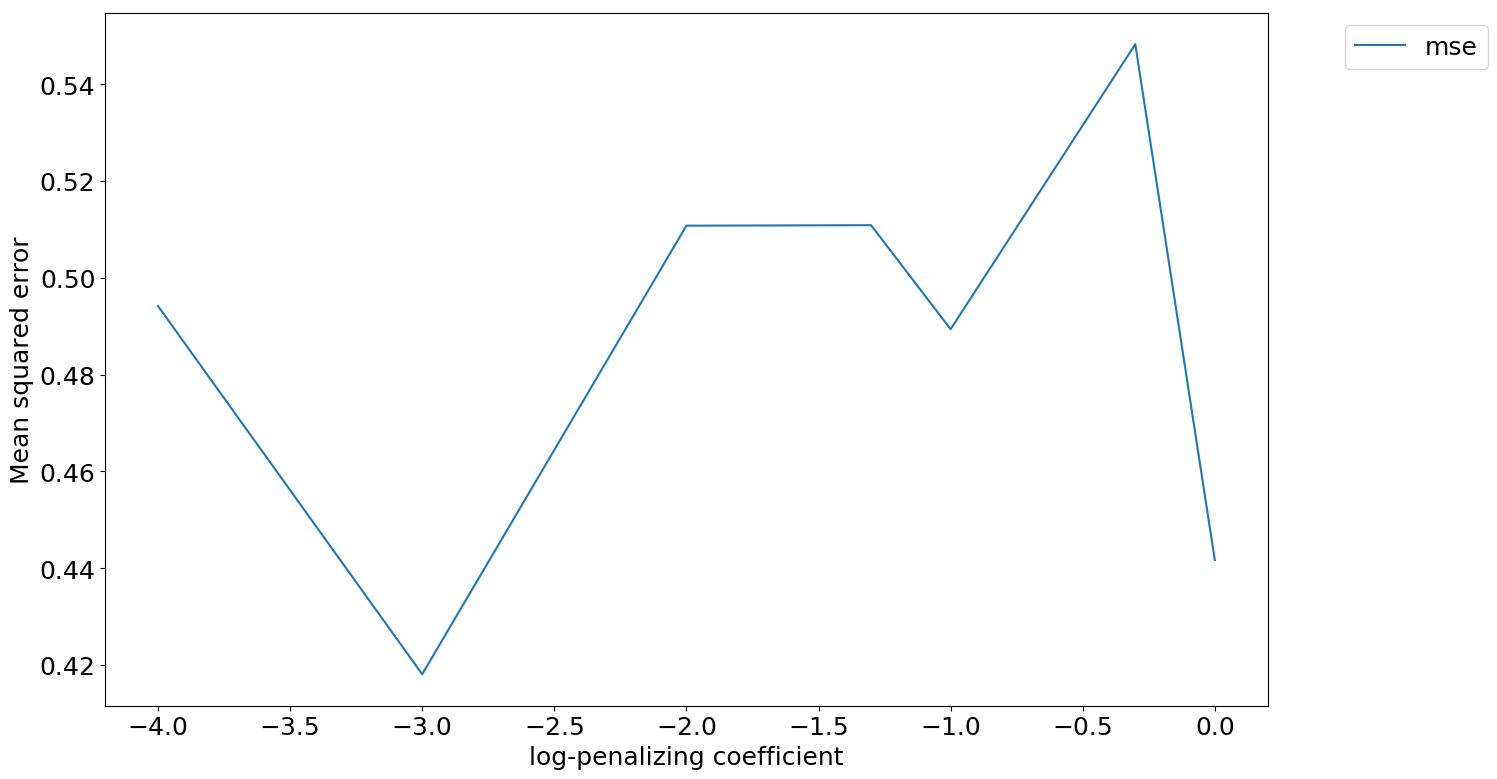
\includegraphics[scale=0.3]{mse-lambda-lasso.png}
    \caption{Lasso mean-squared error vs base-10 log of tuning parameter}
    \label{fig:neurons}
\end{figure}

\noindent The above table indicates that the minimum mean-squared error is obtained when the penalizing coefficient $\lambda$ = 0.001 and the value of the mean squared error is 0.4181. The average overall runtime of the lasso is 28.4 ms.
		\newpage
    	\subsection{Elastic Net}
    	The elastic net utilizes a penalty that involves both, the $\ell_1$ and $\ell_2$ norms, thereby allowing for a better tunability of the model. In this implementation of the elastic net, the ratio between the $\ell_1$ and $\ell_2$ norms is set at 1:1 but can also be tuned as an additional hyper-parameter.
    	\begin{figure}[H]
            \centering
            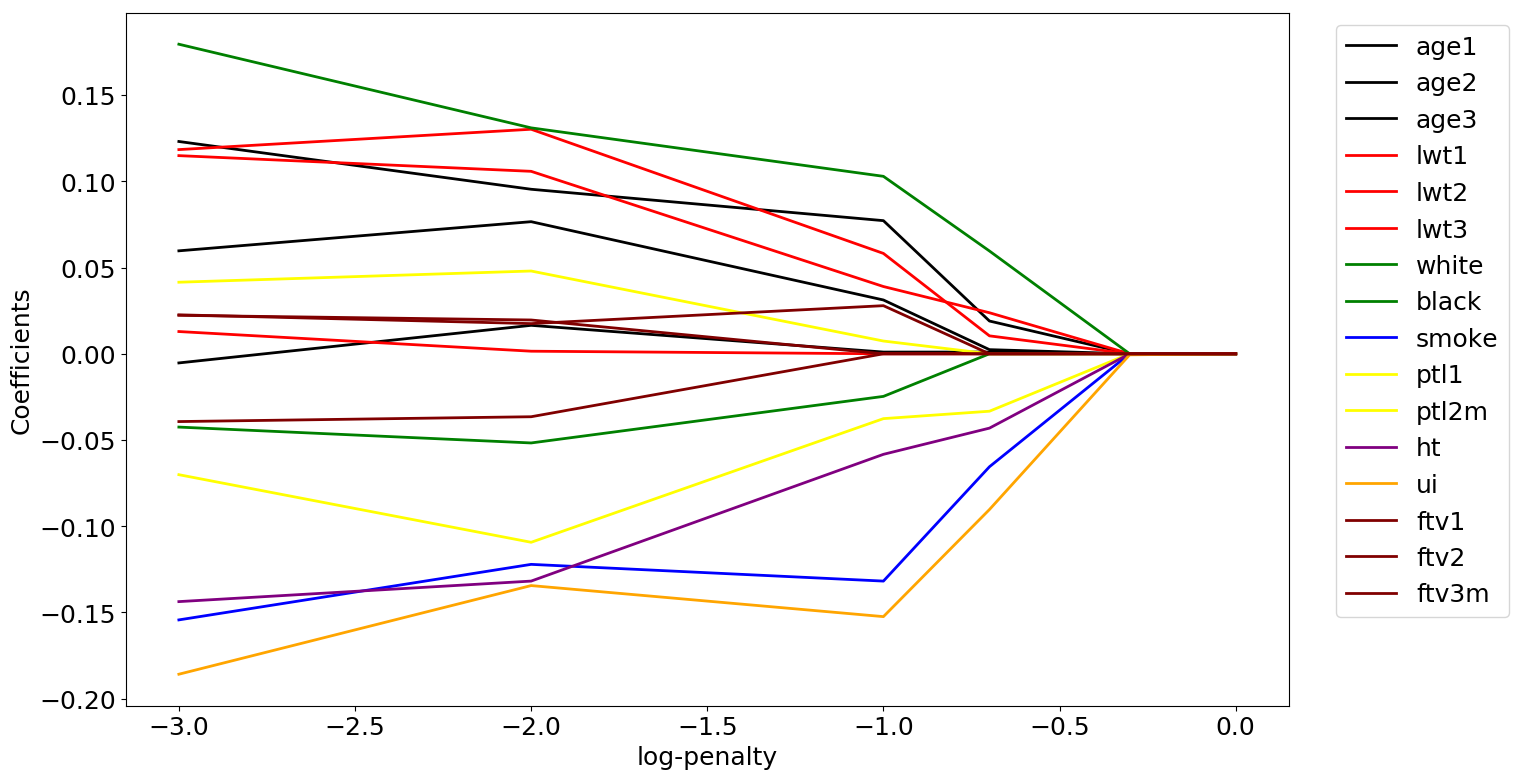
\includegraphics[scale=0.4]{enet-path.png}
            \caption{Elastic net coefficients vs base-10 log of tuning parameter}
            \label{fig:neurons}
        \end{figure}
        \noindent The above figure indicates the sparsity introduced in the model as a function of the base-10 log of the penalizing coefficient. As the penalizing coefficient $\lambda$ increases, more and more coefficients are set to 0. Along with feature selection, the elastic net also penalizes the selected features, thereby leading to shrinkage. This leads to a model that generalizes well.  \\ 
        
        \noindent However, the elastic net penalty, by nature, does not account for group-wise relationships between variables. As a result, the variables elimination process is independent of the group-wise structure of features, leading to unstructured sparsity. The sparsity pattern of the elastic net can be observed in the following table:\\
\begin{table}[H]
\centering
\begin{tabular}{|l|c|c|c|c|c|c|}
\hline
\textbf{penalty}     & \textbf{0.0010} & \textbf{0.0100} & \textbf{0.1000} & \textbf{0.2000} & \textbf{0.5000} & \textbf{1.0000} \\ \hline
\textbf{log-penalty} & -3.0000         & -2.0000         & -1.0000         & -0.6990         & -0.3010         & 0.0000          \\ \hline
\textbf{age1}        & -0.0053         & 0.0165          & 0.0010          & 0.0010          & 0.0000          & 0.0000          \\ \hline
\textbf{age2}        & 0.1231          & 0.0954          & 0.0772          & 0.0190          & 0.0000          & 0.0000          \\ \hline
\textbf{age3}        & 0.0597          & 0.0766          & 0.0312          & 0.0024          & 0.0000          & 0.0000          \\ \hline
\textbf{lwt1}        & 0.1184          & 0.1302          & 0.0582          & 0.0104          & 0.0000          & 0.0000          \\ \hline
\textbf{lwt2}        & 0.0129          & 0.0015          & 0.0000          & 0.0000          & 0.0000          & 0.0000          \\ \hline
\textbf{lwt3}        & 0.1149          & 0.1058          & 0.0390          & 0.0238          & 0.0000          & 0.0000          \\ \hline
\textbf{white}       & 0.1795          & 0.1310          & 0.1029          & 0.0596          & 0.0000          & 0.0000          \\ \hline
\textbf{black}       & -0.0425         & -0.0517         & -0.0247         & 0.0000          & 0.0000          & 0.0000          \\ \hline
\textbf{smoke}       & -0.1543         & -0.1221         & -0.1318         & -0.0655         & 0.0000          & 0.0000          \\ \hline
\textbf{ptl1}        & -0.0701         & -0.1093         & -0.0376         & -0.0333         & 0.0000          & 0.0000          \\ \hline
\textbf{ptl2m}       & 0.0415          & 0.0480          & 0.0074          & 0.0000          & 0.0000          & 0.0000          \\ \hline
\textbf{ht}          & -0.1437         & -0.1318         & -0.0583         & -0.0431         & 0.0000          & 0.0000          \\ \hline
\textbf{ui}          & -0.1858         & -0.1344         & -0.1524         & -0.0903         & -0.0006         & 0.0000          \\ \hline
\textbf{ftv1}        & 0.0226          & 0.0175          & 0.0279          & 0.0000          & 0.0000          & 0.0000          \\ \hline
\textbf{ftv2}        & 0.0223          & 0.0196          & 0.0000          & 0.0000          & 0.0000          & 0.0000          \\ \hline
\textbf{ftv3m}       & -0.0393         & -0.0365         & 0.0000          & 0.0000          & 0.0000          & 0.0000          \\ \hline
\textbf{intercept}   & 2.9584          & 2.9300          & 2.9424          & 2.9418          & 2.9271          & 2.9289          \\ \hline
\textbf{mse}         & 0.4623          & 0.4191          & 0.4018          & 0.4776          & 0.5481          & 0.4153          \\ \hline
\end{tabular}
\caption{Elastic net coefficients as a function of tuning parameter}
\end{table}

\noindent We can also plot the mean-squared error as a function of the tuning parameter to obtain the following graph: 

\begin{figure}[H]
 \centering
 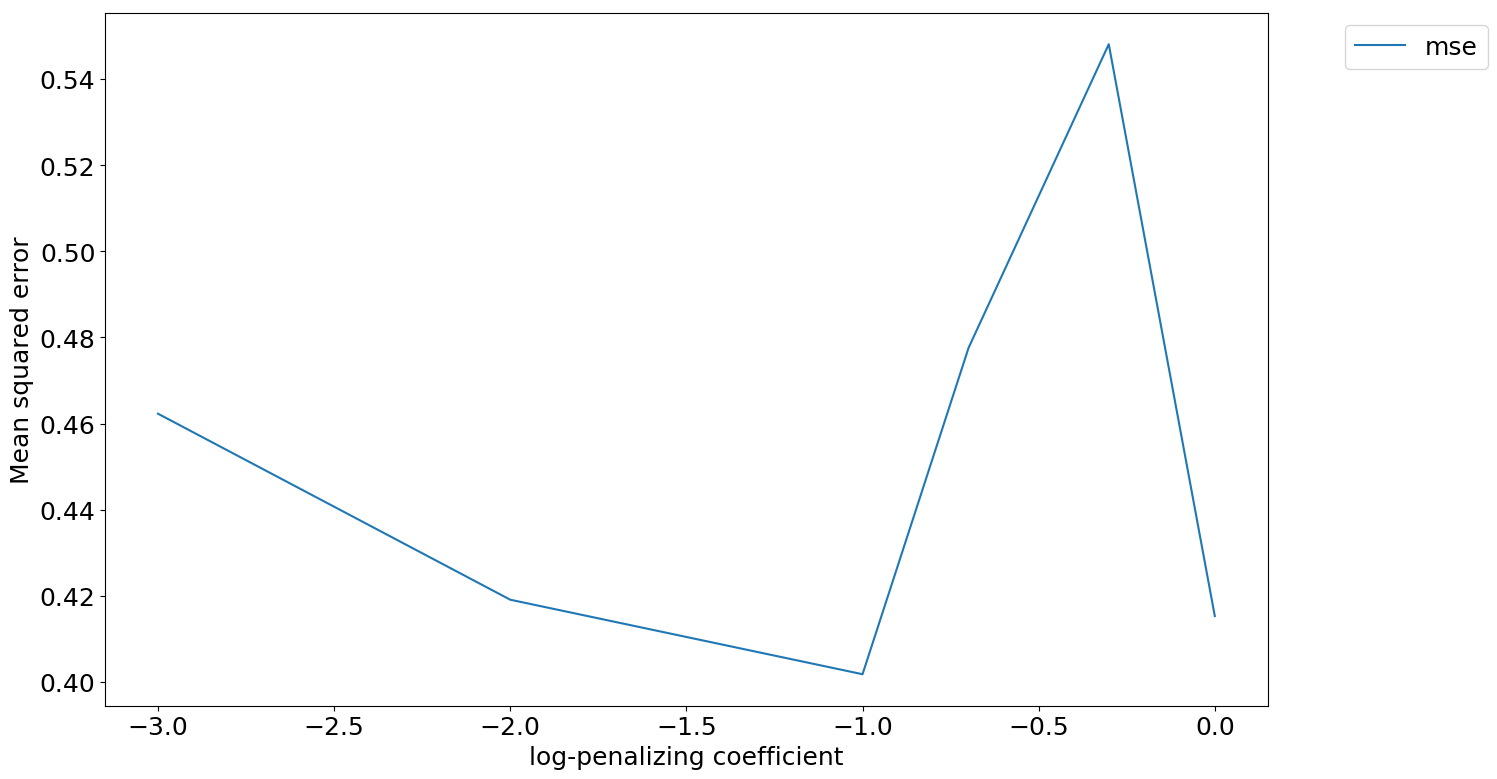
\includegraphics[scale=0.3]{mse-lambda-elastic_net.png}
  \caption{Elastic-net mean-squared error vs base-10 log of tuning parameter}
  \label{fig:neurons}
\end{figure}
It can be seen that the minimum error is achieved at $\lambda$ = 0.1 and the error value is 0.4018. The average overall runtime of the elastic net is found to be 25.8 ms.
\newpage
\subsection{Group Lasso}
The group-lasso allows for specification of feature groups in the penalty, allowing for a model that is interpretable and accounts for relationships between features in the model building process. The coefficients values for all predictors are plotted below as the tuning parameter is varied from 0.001 to 1 in steps of multiples of 10. 
\\
\begin{figure}[H]
 \centering
 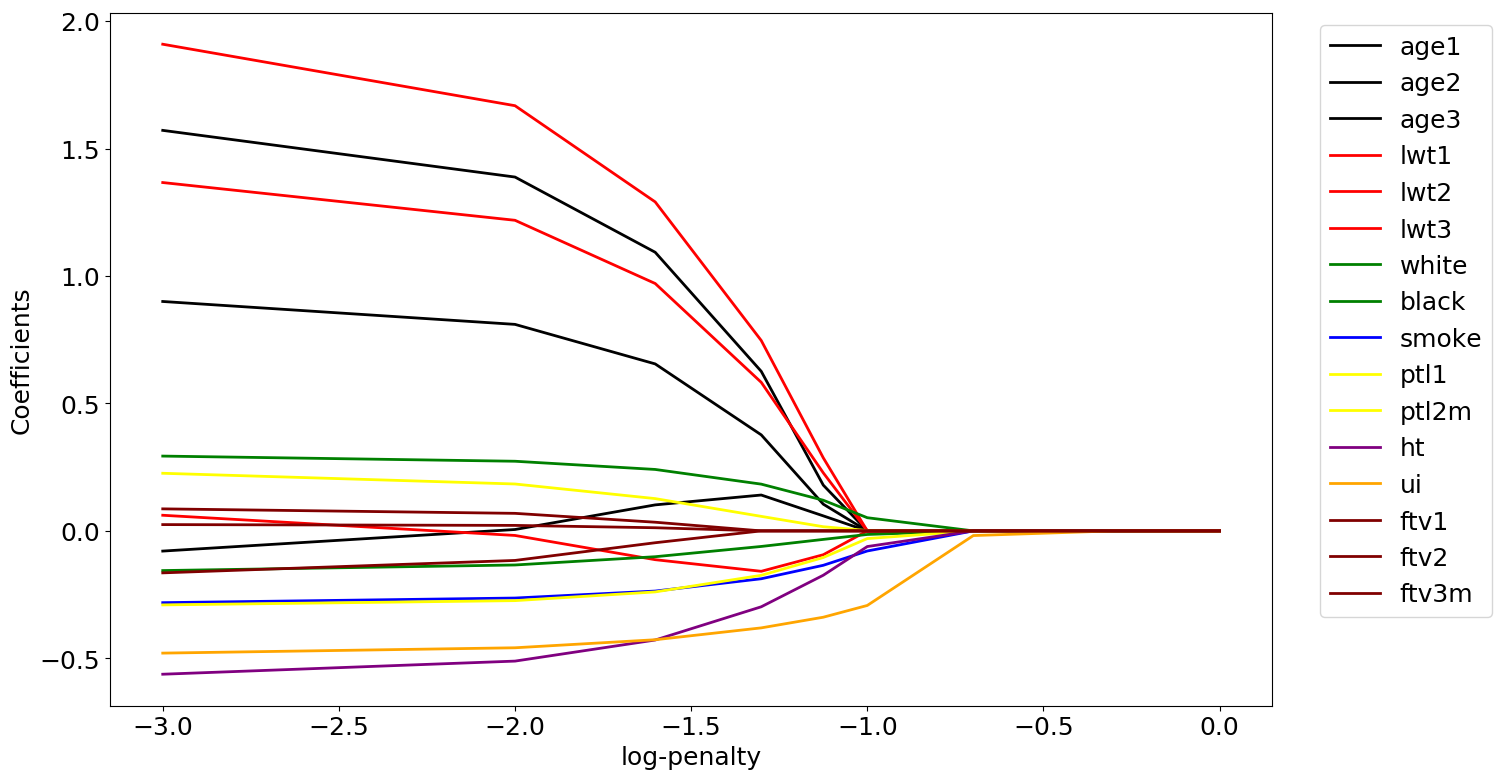
\includegraphics[scale=0.4]{grplasso-path.png}
  \caption{Group lasso coefficients vs base-10 log of tuning parameter}
  \label{fig:neurons}
\end{figure}
\noindent 
The most striking difference between the group lasso and other models discussed earlier in the way in which the predictors are eliminated from the model. We can see from the above graph that coefficients of predictors belonging to a group are simultaneously set to zero as the value of the tuning parameter increases. For example, we can see in the coefficient table below that the first group of variables eliminated from the model is the group corresponding to number of clinician visits. We know that if a visit to the physician does not affect the weight of the infant, two visits or more should also not affect the weight of the infant. While all models discussed earlier fail to capture this insight, the group lasso sets the coefficients corresponding to ftv1, ftv2, ftv3m simultaneuously to zero, producing a model that is easier to interpret.
\begin{table}[H]
\resizebox{\columnwidth}{!}{%
\begin{tabular}{|l|c|c|c|c|c|c|c|c|c|}
\hline
\textbf{penalty}     & \textbf{0.0010} & \textbf{0.0100} & \textbf{0.0250} & \textbf{0.0500} & \textbf{0.0750} & \textbf{0.1000} & \textbf{0.2000} & \textbf{0.5000} & \textbf{1.0000} \\ \hline
\textbf{log-penalty} & -3.0000         & -2.0000         & -1.6021         & -1.3010         & -1.1249         & -1.0000         & -0.6990         & -0.3010         & 0.0000          \\ \hline
\textbf{intercept}   & 3.0487          & 3.0434          & 3.0379          & 3.0289          & 3.0149          & 3.0021          & 2.9473          & 2.9446          & 2.9446          \\ \hline
\textbf{age1}        & -0.0792         & 0.0054          & 0.1020          & 0.1407          & 0.0590          & 0.0000          & 0.0000          & 0.0000          & 0.0000          \\ \hline
\textbf{age2}        & 1.5714          & 1.3883          & 1.0931          & 0.6260          & 0.1796          & 0.0000          & 0.0000          & 0.0000          & 0.0000          \\ \hline
\textbf{age3}        & 0.9001          & 0.8102          & 0.6551          & 0.3767          & 0.1049          & 0.0000          & 0.0000          & 0.0000          & 0.0000          \\ \hline
\textbf{lwt1}        & 1.9094          & 1.6682          & 1.2907          & 0.7470          & 0.2866          & 0.0000          & 0.0000          & 0.0000          & 0.0000          \\ \hline
\textbf{lwt2}        & 0.0614          & -0.0179         & -0.1129         & -0.1585         & -0.0935         & 0.0000          & 0.0000          & 0.0000          & 0.0000          \\ \hline
\textbf{lwt3}        & 1.3667          & 1.2186          & 0.9706          & 0.5829          & 0.2278          & 0.0000          & 0.0000          & 0.0000          & 0.0000          \\ \hline
\textbf{white}       & 0.2935          & 0.2733          & 0.2411          & 0.1835          & 0.1203          & 0.0517          & 0.0000          & 0.0000          & 0.0000          \\ \hline
\textbf{black}       & -0.1556         & -0.1337         & -0.1013         & -0.0610         & -0.0334         & -0.0140         & 0.0000          & 0.0000          & 0.0000          \\ \hline
\textbf{smoke}       & -0.2816         & -0.2635         & -0.2361         & -0.1878         & -0.1350         & -0.0788         & 0.0000          & 0.0000          & 0.0000          \\ \hline
\textbf{ptl1}        & -0.2903         & -0.2736         & -0.2394         & -0.1743         & -0.1045         & -0.0301         & 0.0000          & 0.0000          & 0.0000          \\ \hline
\textbf{ptl2m}       & 0.2261          & 0.1840          & 0.1267          & 0.0570          & 0.0164          & 0.0014          & 0.0000          & 0.0000          & 0.0000          \\ \hline
\textbf{ht}          & -0.5623         & -0.5109         & -0.4281         & -0.2977         & -0.1740         & -0.0614         & 0.0000          & 0.0000          & 0.0000          \\ \hline
\textbf{ui}          & -0.4795         & -0.4586         & -0.4270         & -0.3805         & -0.3387         & -0.2925         & -0.0183         & 0.0000          & 0.0000          \\ \hline
\textbf{ftv1}        & 0.0864          & 0.0688          & 0.0340          & 0.0000          & 0.0000          & 0.0000          & 0.0000          & 0.0000          & 0.0000          \\ \hline
\textbf{ftv2}        & 0.0247          & 0.0215          & 0.0124          & 0.0000          & 0.0000          & 0.0000          & 0.0000          & 0.0000          & 0.0000          \\ \hline
\textbf{ftv3m}       & -0.1647         & -0.1159         & -0.0465         & 0.0000          & 0.0000          & 0.0000          & 0.0000          & 0.0000          & 0.0000          \\ \hline
\textbf{mse}         & 0.4332          & 0.4196          & 0.4377          & 0.4560          & 0.4713          & 0.4961          & 0.5299          & 0.5329          & 0.5329          \\ \hline
\end{tabular}
}
\caption{Group-lasso coefficients as a function of tuning parameter}
\end{table}
\noindent We can also plot the mean-squared error as a function of the base-10 log of the tuning parameter to obtain the following graph:
\begin{figure}[H]
 \centering
 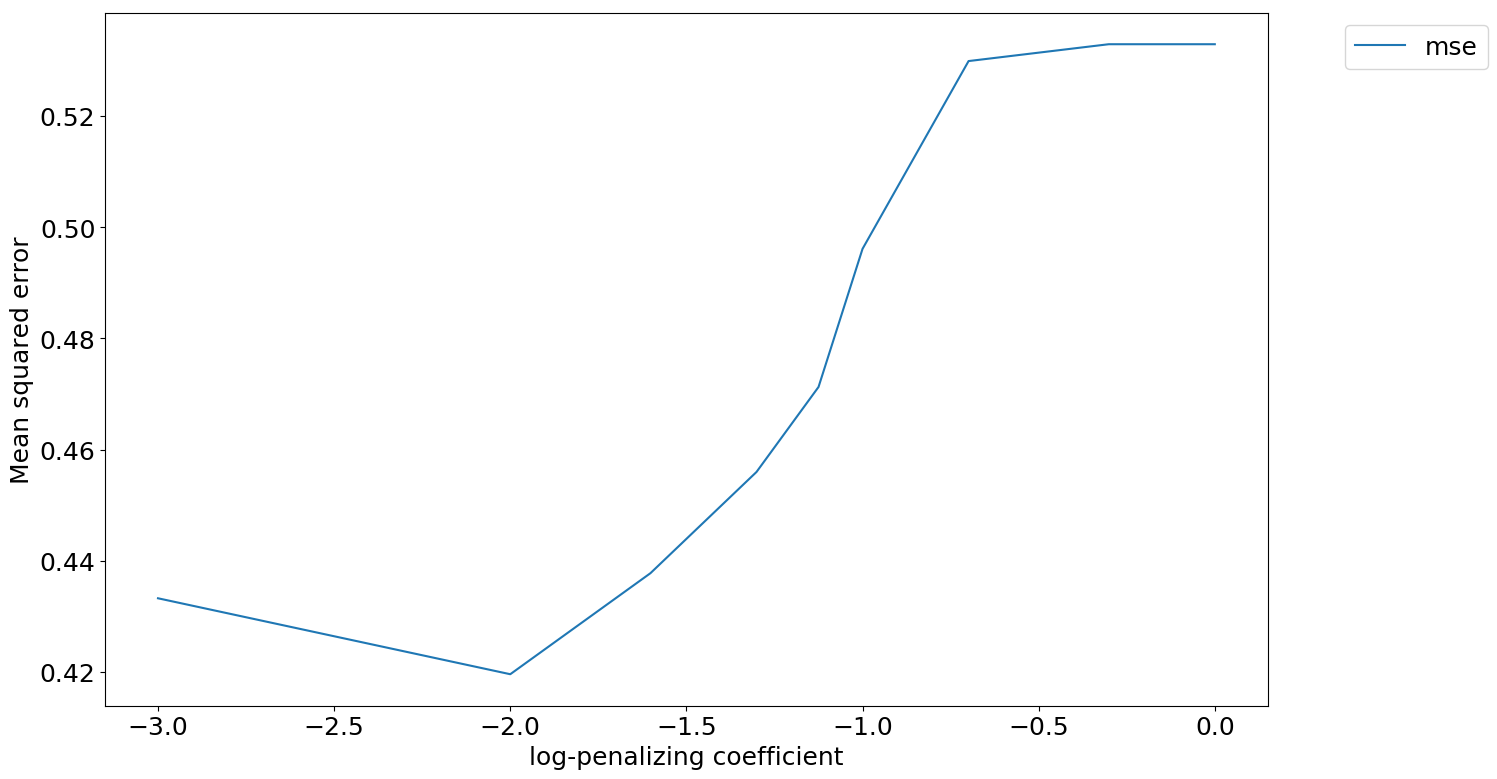
\includegraphics[scale=0.3]{mse-lambda-grplasso.png}
  \caption{Mean-squared error vs base-10 log of tuning parameter}
  \label{fig:neurons}
\end{figure}
\noindent We can see that the minimum value for mean-squared error is obtained when the tuning parameter $\lambda$ = 0.01 and the value of the error is 0.4196. This is slightly higher than the error value obtained from the elastic net. The average overall runtime of the group-lasso is 74.0 ms.

\newpage

\newpage
\subsection{ALAMO}
We can analyze which features are included in the model as a function of each ALAMO iteration. The following table shows the feature subsets and mean-squared error as ALAMO iterations progress:

\begin{table}[H]
\centering
\resizebox{\textwidth}{!}{%
\begin{tabular}{|c|l|l|}
\hline
\textbf{Iteration  \#} & \multicolumn{1}{c|}{\textbf{Feature subsets}}                  & \multicolumn{1}{c|}{\textbf{MSE}} \\ \hline
1                      & (age1, age2, age3, lwt1, lwt2, lwt3, white)                    & 4.37                              \\ \hline
2                      & (age1, age2, age3, lwt1, lwt2, lwt3, white,1)                  & 0.472                             \\ \hline
3                      & (age1, age2, age3, lwt1, lwt2, lwt3, white, ui, 1)             & 0.444                             \\ \hline
4                      & (age1, age2, age3, lwt1, lwt2, lwt3, white, ht,  ui, 1)        & 0.420                             \\ \hline
5                      & (age1, age2, age3, lwt1, lwt2, lwt3, white, smoke, ht,  ui, 1) & 0.402                             \\ \hline
\end{tabular}
}
\caption{Solution paths of ALAMO}

\end{table}

\noindent The linear model obtained from ALAMO is as follows:
\\

\begin{center}
    \textit{Y (predicted) = - 0.23 * age1 + 1.5 * age2 + 1.1 * age3 + 1.7 * lwt1 + 0.23 * lwt2 + 1.3 * lwt3 + 0.40 * white - 0.36 * smoke - 0.60 * ht - 0.50 * ui + 3.0}
\end{center}

\\



\noindent We can observe that ALAMO renders the model with the fewest terms as compared with the previous models, while maintaining group-wise relationships between predictors. It also achieves a mean-squared error lower than the group-lasso and comparable with the elastic-net. ALAMO achieves structured sparsity among predictors as apposed to unstructured sparsity with the elastic net. The overall result is a model that contains the fewest terms while maintaining a low generalization error and accounts for constraints among predictors and predictor-groups. \\

\noindent While ALAMO converges in fewer iterations as compared to other algorithms, each ALAMO iteration is computationally expensive, owing to the non-convexity of the subset selection problem. As a result, the average overall runtime of ALAMO is 334.0 ms and is slower than the models described earlier.
\newpage
\section{Conclusion}
The following table summarizes the results from the multiple models used for fitting the data:
\begin{table}[H]
\begin{tabular}{|l|c|c|c|}
\hline
\textbf{Model}    & \multicolumn{1}{l|}{\textbf{Mean-squared error}} & \multicolumn{1}{l|}{\textbf{Average Runtime (ms)}} & \multicolumn{1}{l|}{\textbf{Number of terms}} \\ \hline
Linear regression & 0.4825                                           & 5.9                                                & 16                                            \\ \hline
Ridge             & 0.4235                                           & 43.1                                               & 16                                            \\ \hline
Lasso             & 0.4181                                           & 28.4                                               & 16                                            \\ \hline
Elastic net       & 0.4018                                           & 25.8                                               & 13                                            \\ \hline
Group lasso       & 0.4196                                           & 74.0                                               & 16                                            \\ \hline
ALAMO             & 0.4020                                           & 334.0                                              & 11                                            \\ \hline
\end{tabular}
\end{table}
\noindent We can see that linear regression contains 16 terms and has the highest generalization error due to overfitting on the training data. However, being the simplest model to train, linear regression is the fastest and has an average total runtime  of 5.9 ms.\\

\noindent The ridge attempts to fix the problem of overfitting by shrinking the coefficients and this can be seen by the lower mean-squared error of the ridge over the simple linear regression model. The ridge does not remove predictors from the model and hence the number of terms is still 16. As it solves the additional convex penalty term, the ridge takes longer to run than the linear regression model and this is evident from the runtime results. \\

\noindent The lasso gives a mean-squared error lower than the ridge and linear regression when the number of terms included is 16. However, as the model gets sparser, the error goes on increasing due to underfitting. Here, the trade-off between model interpretability and model accuracy comes into picture. Intuitively, the terms corresponding to the number of clinician visits should be excluded from the model, but doing so leads to an increase in mean-squared error if the lasso is used for feature selection. \\

\noindent The elastic net serves as an intermediate penalty between the lasso and the ridge and accounts for both, variable shrinkage and selection. It gives a lower mean-squared error than lasso, ridge and linear regression as it allows for better tunability and incorporates shrinkage and selection. It leads to a model with 13 terms. However, the elastic net and the lasso do not account for incorporation of prior knowledge about the group-wise nature of predictors in the model building process. \\

\noindent The group lasso accounts for the group-wise relationship between the predictors. The lowest mean-squared error from the group-lasso is higher than that of the elastic net due to the constraint that individual variables cannot be removed from the model, thus leading to a slightly higher error at the advantage of better model interpretability. As the penalty is increased, the number of terms in the group-lasso decreases but the error increases due to underfitting. The runtime of the group lasso is also higher than that of other GLMs due to the complexity of the penalty term.\\

\noindent The best-subset strategy of ALAMO gives a mean-squared error of 0.402 and leads to a model with 11 terms. Owing to manual specification of constraints on variables and variable groups, ALAMO leads to a model that is more interpretable and allows for better control by incorporating prior knowledge and insight about features and feature relationships. Owing to the non-convex penalty that ALAMO tries to solve, the runtime of ALAMO is greater than GLMs discussed earlier. \\

\noindent All models discussed above have their unique characteristics. The group lasso and ALAMO are two models that allow for defining feature relationships that can be utilized in the model building process. The group lasso incorporates structured sparsity-based regularization and allows for variable and group specification. However, the group selection is entirely dependent on a single tuning parameter and poses limitations in terms of defining complex relationships between predictors. ALAMO, on the other hand, allows for specification of group-constraints at a predictor-level and also accounts for constraints on the presence and absence of certain groups of predictors in the model. This leads to a lower error and higher control on the model in comparison with the group-lasso at the cost of higher runtime. Additionally, ALAMO allows for non-linear transformations of the predictors, allowing for learning more complex functions from data. However, this analysis is beyond the scope of this work. \\

\newpage
% \nocite{*}

% \bibliography{bibliography} 
% \bibliographystyle{ieeetr}
\bibliographystyle{ieeetr}
\printbibliography
}
\end{document}
